\chapter{SP2-CU1 Consultar contenido de propuesta de Unidad de Aprendizaje}

\begin{UseCase}{SP2-CU2}{ Consultar contenido de propuesta de Unidad de Aprendizaje}{El usuario jefe de desarrollo e innovación curricular, analista y jefe de la división de innovación académica podrán consultar los contenidos de las unidades de aprendizaje de la unidad académica correspondiente.}
		\UCitem{Versión}{\color{Gray}1.0}
		\UCitem{Autor}{\color{Gray}Parra Garcilazo Cinthya Dolores}
		\UCitem{Supervisa}{\color{Gray}}
		\UCitem{Actor}{\hyperlink{Usuario}{Jefe de Desarrollo e Innovación Curricular, analista y Jefe de la División de Innovación Académica}}
		\UCitem{Propósito}{Verificar que el contenido que fue llenado por el capital humano de la unidad académica correspondiente pueda ser aprobado o cuene con áreas de oportunidad.}
		\UCitem{Entradas}{Las entradas para consultar una propuesta de unidades de aprendizaje son:
          \begin{itemize}
          	\item Unidad Académica
            \item Programa académico
		\item Semestre
		\item Número de revisión
          \end{itemize}
        }
		\UCitem{Origen}{Teclado, mouse.}
		\UCitem{Salidas}{
        	\begin{itemize}
        	   \item MSG25. Ha ocurrido un error con la base de datos.

        	\end{itemize}
        }
		\UCitem{Destino}{Pantalla.}
		\UCitem{Precondiciones}{ 
			\begin{itemize}
        	   \item El usuario debe estar autorizado para acceder a dicha unidad de aprendizaje.
		   \item 

        	\end{itemize}
		}
		\UCitem{Postcondiciones}{Se visualiza el paquete de unidades de aprendizaje de un semestre en particular, elegido por el usuario.}
		\UCitem{Errores}{No hay conexión con la base de datos.}
		\UCitem{Estado}{Aprobado.}
		\UCitem{Observaciones}{}
\end{UseCase}

%--------------------------- CU TRAYECTORIA PRINCIPAL -------------------------
\begin{UCtrayectoria}{Principal}


    \UCpaso Muestra la interfaz de usuario Consulta tareas \IUref{xxxxx} %no tengo la vista.
    \UCpaso [\UCactor] Selecciona el botón \IUbutton {Ir A} de la unidad de aprendizaje que quiera consultar. \hyperref[SP2-CU1-A]{Trayectoria A}.
    \UCpaso  Muestra la interfaz de usuario \IUref{Inicio}.

\end{UCtrayectoria}


%------------------------ CU TRAYECTORIA ALTERNARIVA A -------------------------
\label{SP2-CU1-A}
\begin{UCtrayectoriaA}{A}{El usuario no tiene el permiso para acceder a la unidad de aprendizaje.}
    \UCpaso Muestra el mensaje MSG24. Por el momento la página solicitada no esta disponible
    \UCpaso[\UCactor] Presiona el botón \IUbutton {Aceptar}
\end{UCtrayectoriaA}

%------------------------ Pantallas de este caso de uso -------------------------
\chapter{Pantallas}
 \begin{figure}
  \centering
    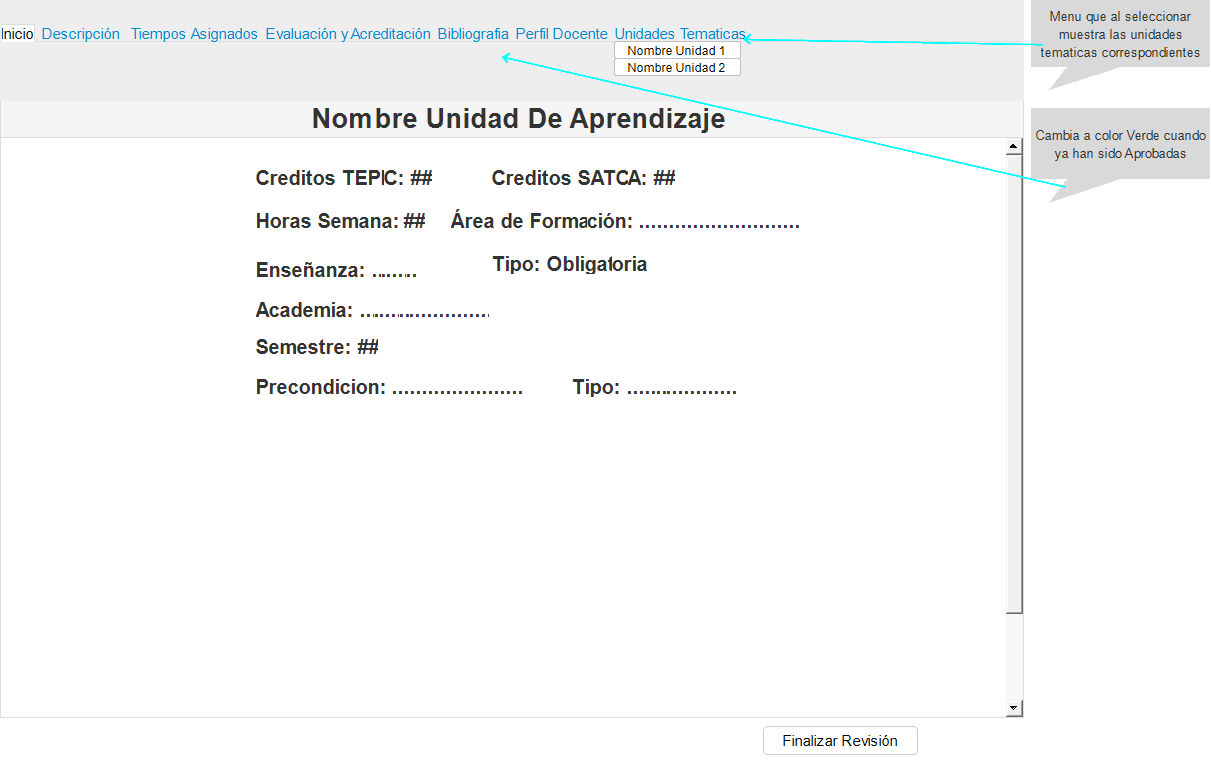
\includegraphics[width=0.7\textwidth]{DCU/SP2/Pantallas/Inicio}
  \caption{SP2-IU-ConsultaPaquete}
  \label{SP2-IU-ConsultaPaquete}
\end{figure}


